\documentclass[../main.tex]{subfiles}
\usepackage{graphicx} % Required for including images

\setstretch{0.1} % Adjust spacing for readability

\begin{document}
{\let\clearpage\relax\chapter{Results}}
\vspace{-5pt}

\section{Simulation of an Optical Flat}
\vspace{-15pt}
The evaluation of both ray-tracing and wavefront simulation models in the simulation of optical flats has demonstrated that the integration of these methods provides a clear depiction of optical behaviors. Ray-tracing accurately models the interactions of light waves with optical flats, reflecting the inherent properties of materials and nuances of surface quality. Altough the ray-tracing engine worked, this result was not achieved in this bachelorthesis. Complementary to this, wavefront simulations effectively visualized the propagation and interference of light waves as they interact with surfaces.
\vspace{-15pt}
\subsection{Simulation Results}
\begin{minipage}{\textwidth}
\begin{wrapfigure}{l}{0.3\textwidth}
    \centering
    \vspace{-0.8cm}
    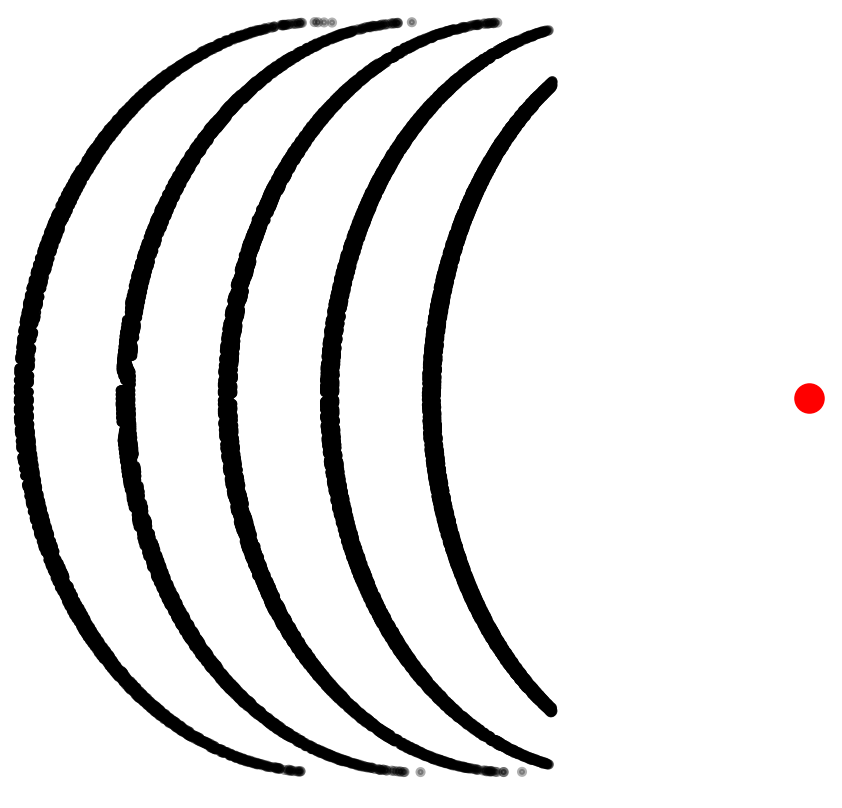
\includegraphics[width=0.3\textwidth]{Images/Results/optical_flat_visualization4}
    \caption{Simulated interference pattern generated by the application. The red dot depicts the place of the hinge of the optical flat. More fringes and more continuity in the fringes can be achieved by adjusting the \texttt{num\_disks} and the \texttt{resolution} parameters.}
    \label{fig:interference}
\end{wrapfigure}
The simulation functionalities within the application were tested to analyze their performance in replicating realistic scenarios. Through the use of the Python-based simulation modules, we were able to perform intersection and visualize interference patterns. Figure \ref{fig:interference} shows a typical simulation output, illustrating the precision and clarity achieved.
\section{Extraction of 3D Surface Shape from Measurements}
Employing the Fourier Transform (FT) method to extract 3D shapes from optical measurements was the key factor to achieve this result. This technique captures fringe patterns embedded with high-frequency carrier fringes and applies Fourier transform techniques to isolate these fringes and recover detailed phase information. The efficacy of this approach is showcased by its ability to convert interference patterns into quantifiable 3D surface maps.

The integration of phase unwrapping and height map calculation features within the GUI simplifies data processing and reduces the time required for analysis. This functionality facilitates the direct transformation of phase data into 3D topographical maps.
\end{minipage}
\subsection{Surface Topography Visualization}
\vspace{-15pt}
The GUI's 3D view tab provides an interactive visualization of reconstructed surfaces. We could manipulate the view to better understand the topographical details of the surface being studied. An example of a reconstructed surface is shown in Figure \ref{fig:topography}.\\
\begin{figure}[H]
    \centering
    %\hspace{4cm}
    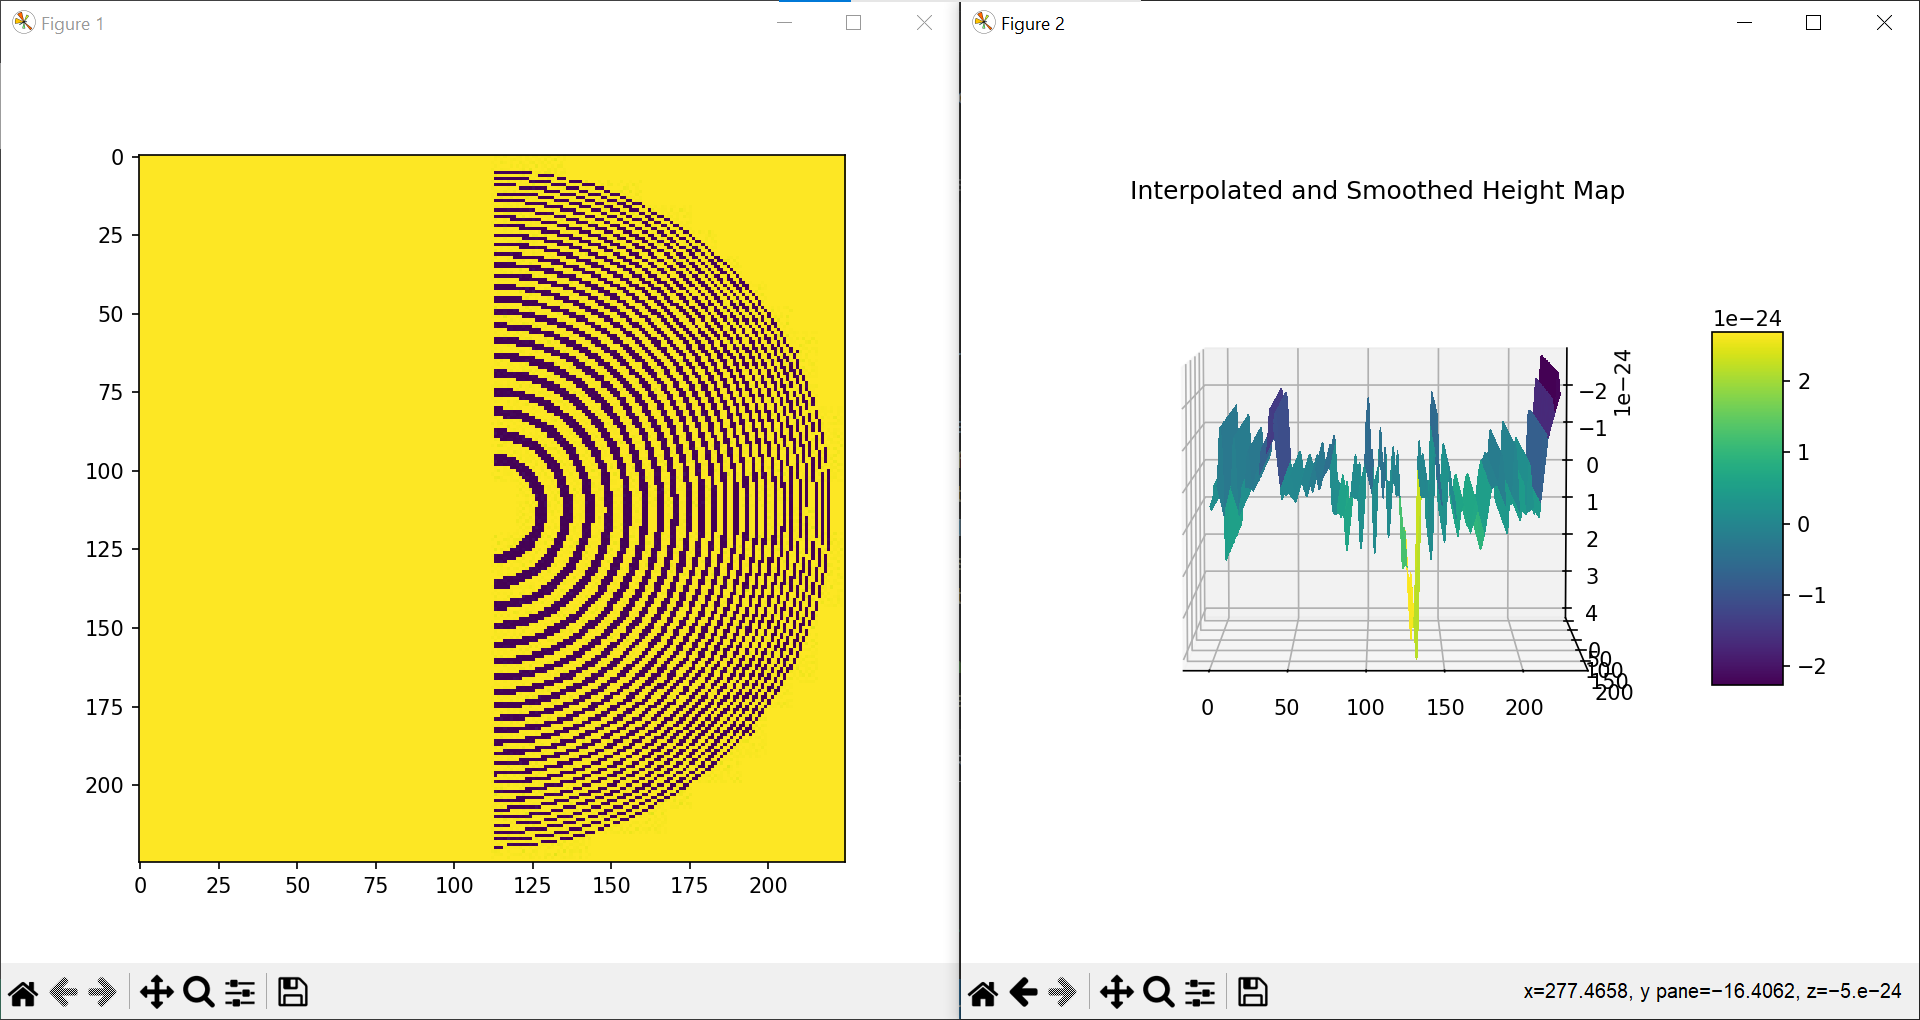
\includegraphics[width=0.6\textwidth]{Images/Results/3D_reconstructie}
    %\hspace{2cm}
    \caption{3D visualization of surface topography as reconstructed by the application.}
    \label{fig:topography}
\end{figure}
\vspace{-15pt}
\section{User Interaction and GUI Performance}
\vspace{-15pt}
The modular design of the GUI proved to be highly effective in facilitating user interaction with datasets and processing tools. The application's responsiveness and stability during high-computation tasks were also good.
\vspace{-15pt}
\section{Representativeness of Simulation and Reconstruction}
\vspace{-15pt}
The representativeness of the simulations and reconstructions was not evaluated due to lack of time. %This could be done by comparing the generated models and extracted data against known standards and real samples. This evaluation indicates that the methods are designed to minimize errors and enhance the accuracy of the simulations. Iterative testing and refining of the simulation parameters should show that they closely align with actual measurements.


\end{document}
